\documentclass[aspectratio=169, 10pt]{beamer}

% --- Theme Setup ---
\usetheme{metropolis}

% --- Colors (University of Innsbruck Approximation) ---
\definecolor{uibkblue}{RGB}{0, 51, 102}    % Dark Blue
\definecolor{uibkorange}{RGB}{233, 131, 0} % Orange

\setbeamercolor{frametitle}{bg=uibkblue, fg=white}
\setbeamercolor{alerted text}{fg=uibkorange}
\setbeamercolor{progress bar}{fg=uibkorange, bg=uibkblue!20}
\setbeamercolor{block title}{bg=uibkblue, fg=white}

% --- Packages ---
\usepackage{booktabs}   % For professional tables
\usepackage{graphicx}   % For images
\usepackage{caption}
\usepackage{subcaption}
\usepackage{tikz}       % For positioning logos

% --- Metadata ---
\title{Hand Gesture Recognition with CNNs}
\subtitle{Visual Computing Project}
\author{Tim Dedie \& Nick Somitsch}
\institute{University of Innsbruck}
\date{January 27, 2026}

\begin{document}

% --- Slide 1: Title Slide ---
{
\setbeamercolor{background canvas}{bg=white}
\begin{frame}
    \titlepage
    % Manually positioning logos
    \begin{tikzpicture}[remember picture, overlay]

    \node[anchor=south east] at (current page.south east) {
            % Using generic name 'uibknew' allows latex to pick the eps or converted pdf
            \includegraphics[height=1.2cm]{images/uibknew} \hspace{0.5cm}
            \includegraphics[height=1.0cm]{images/igslogo.png} \hspace{0.2cm}
            \includegraphics[height=1.0cm]{images/iislogo.png}
        };
 \end{tikzpicture}
\end{frame}
}

% --- Slide 2: Project Overview ---
\begin{frame}{Project Overview}
    \begin{columns}[T, onlytextwidth] % Switched back to [T] (top) alignment to control vertical space manually
        \column{0.45\textwidth}
            % --- Added spacing here to lower the text block ---
            \vspace{0.5cm}
            \textbf{Goal:} Classify hand gestures from webcam input.
            \vspace{0.3cm}

            \textbf{5 Gesture Classes:}
            \begin{itemize}
                \item Thumbs Up / Thumbs Down
                \item Peace Sign
                \item Open Palm
                \item No Hand (background)
            \end{itemize}

            \vspace{0.5cm}
            \textbf{Tech Stack:}
            \begin{itemize}
                \item PyTorch (deep learning)
                \item OpenCV (image processing)
                \item MediaPipe (hand detection)
            \end{itemize}

        \column{0.50\textwidth}
            \centering
            % Added top spacing to image as well to align visually
            \vspace{0.2cm}
            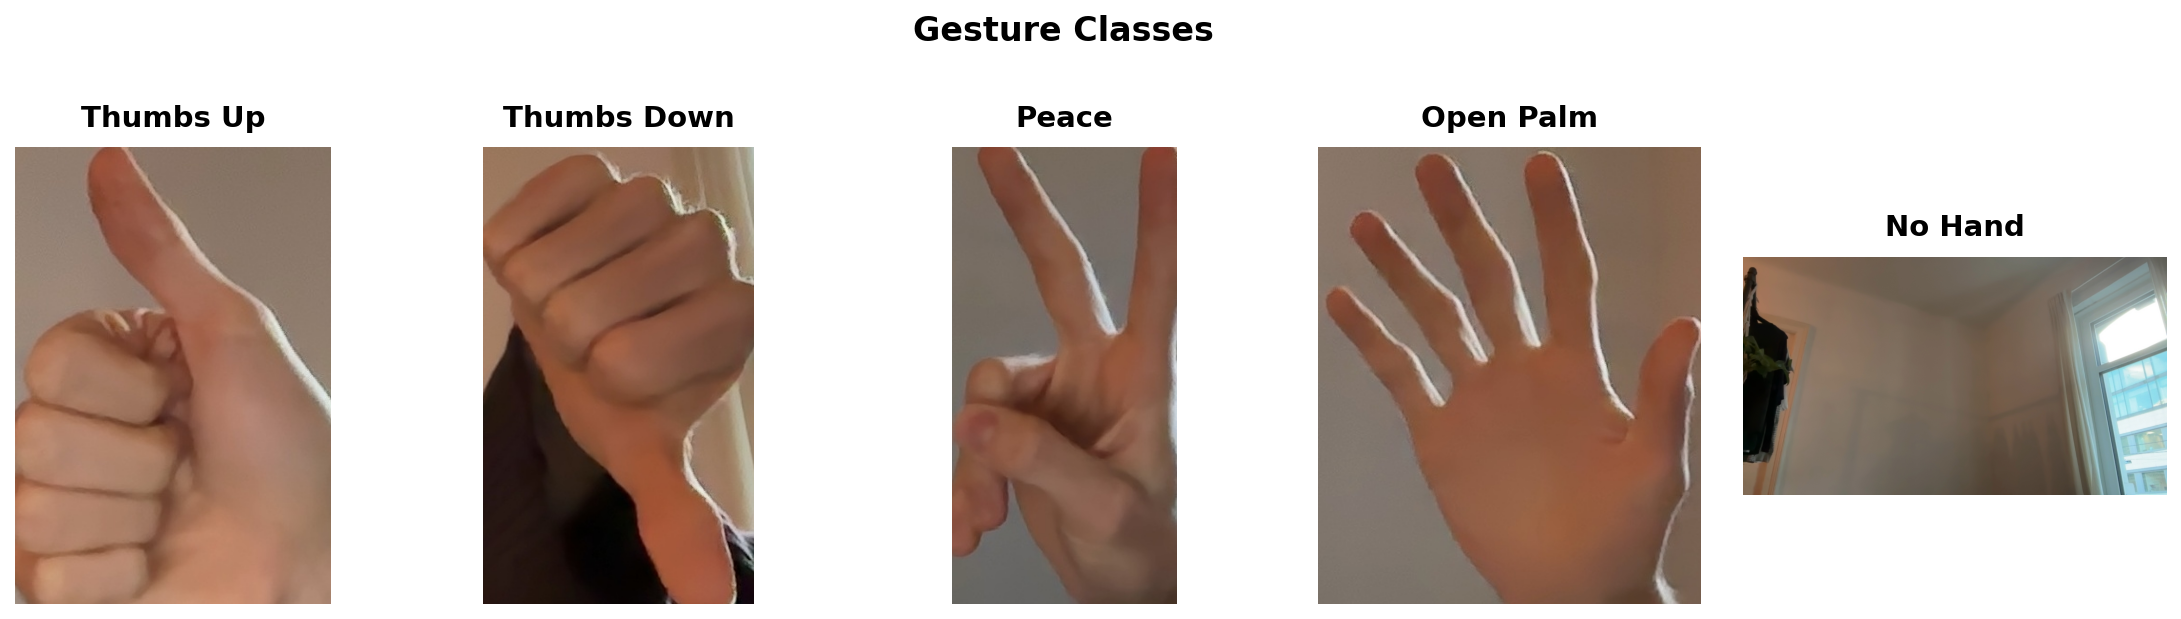
\includegraphics[width=\textwidth]{images/gesture_samples.png}
            \captionof*{figure}{\footnotesize Sample Gestures}
    \end{columns}
\end{frame}

% --- Slide 3: The Problem ---
\begin{frame}{The Problem: Learning Backgrounds}
    \begin{columns}[c, onlytextwidth]
        \column{0.5\textwidth}

             \textbf{Initial Approach:}
            \begin{itemize}
                \item Fed full webcam frames to CNN.
            \end{itemize}

            \vspace{0.3cm}
            \textbf{What Happened:}
            \begin{itemize}
                \item Model learned \alert{backgrounds}, not gestures.
                \item \textit{``Bookshelf = Thumbs Up''}
                \item High training accuracy, poor generalization.
            \end{itemize}

            \vspace{0.3cm}
            \textbf{Root Cause:}
            \begin{itemize}
                \item CNN found easier patterns (room features) than actual hand shapes.
            \end{itemize}

        \column{0.45\textwidth}
            \centering
            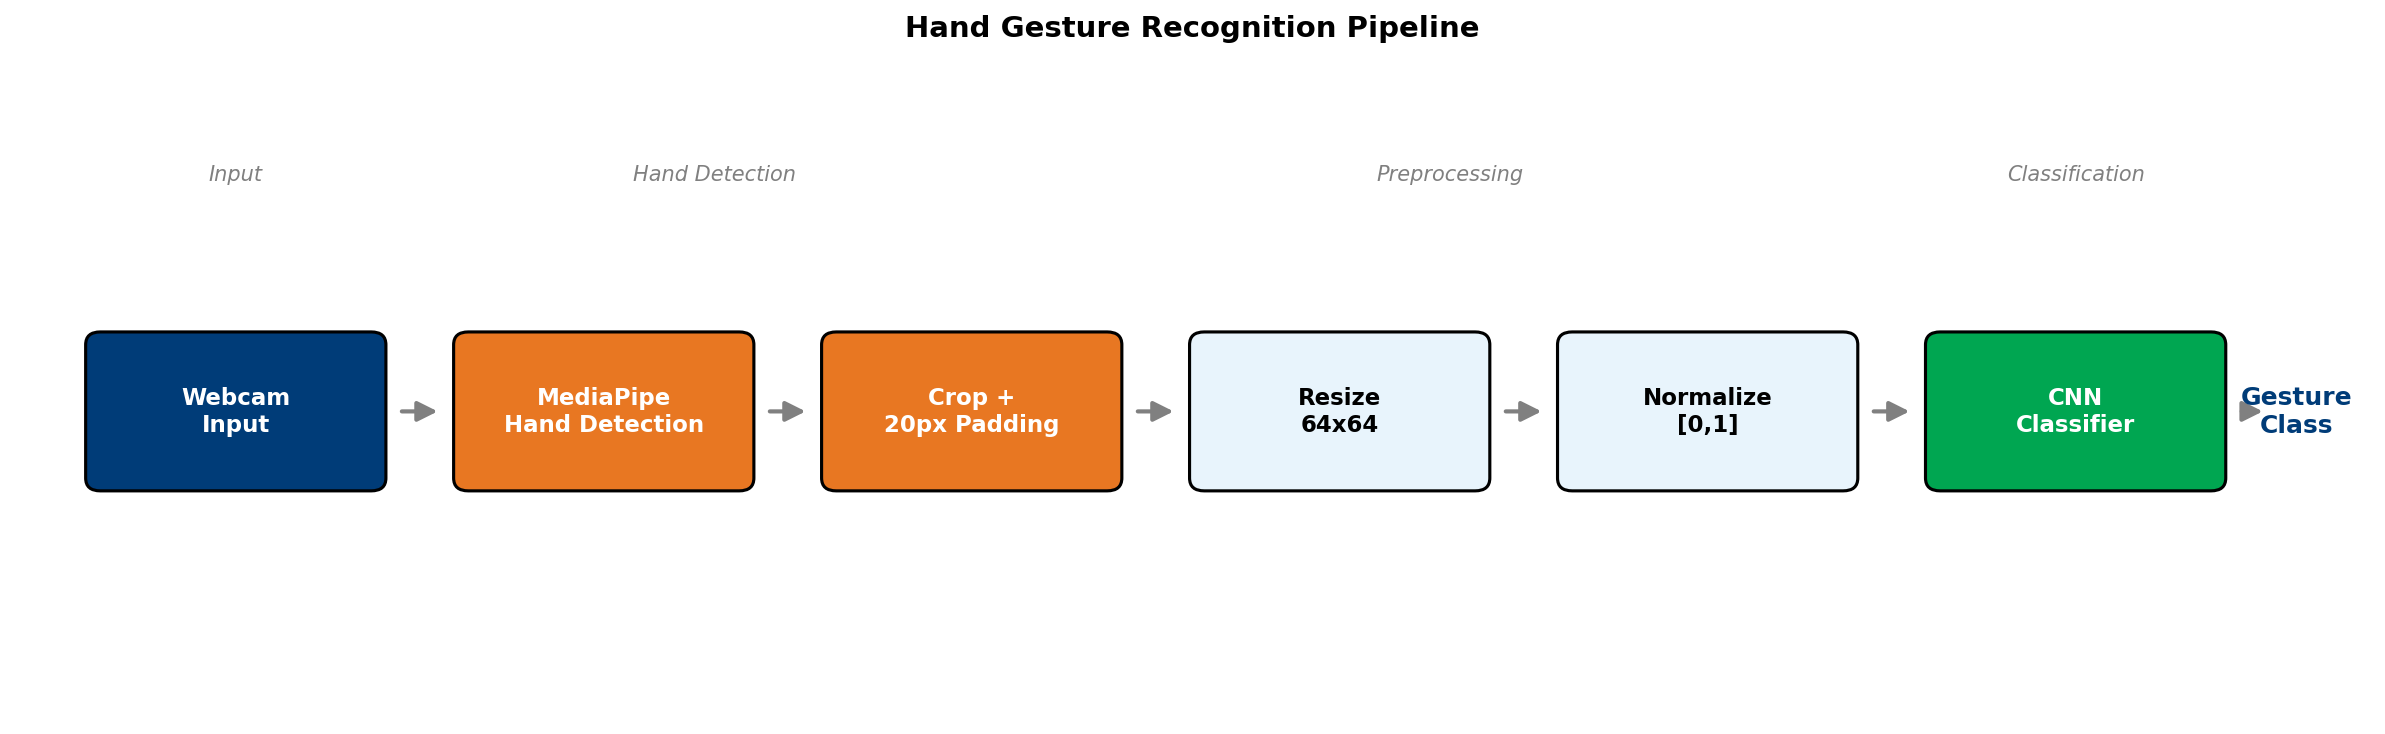
\includegraphics[width=\textwidth]{images/pipeline.png}
            \vspace{1.5em}

            \textbf{\textcolor{uibkorange}{Solution:}} \\
            \large Isolate the hand region first.

    \end{columns}
\end{frame}

% --- Slide 4: The Solution ---
\begin{frame}{The Solution: MediaPipe Hand Cropping}
    % Pipeline image now takes full width
    \centering
    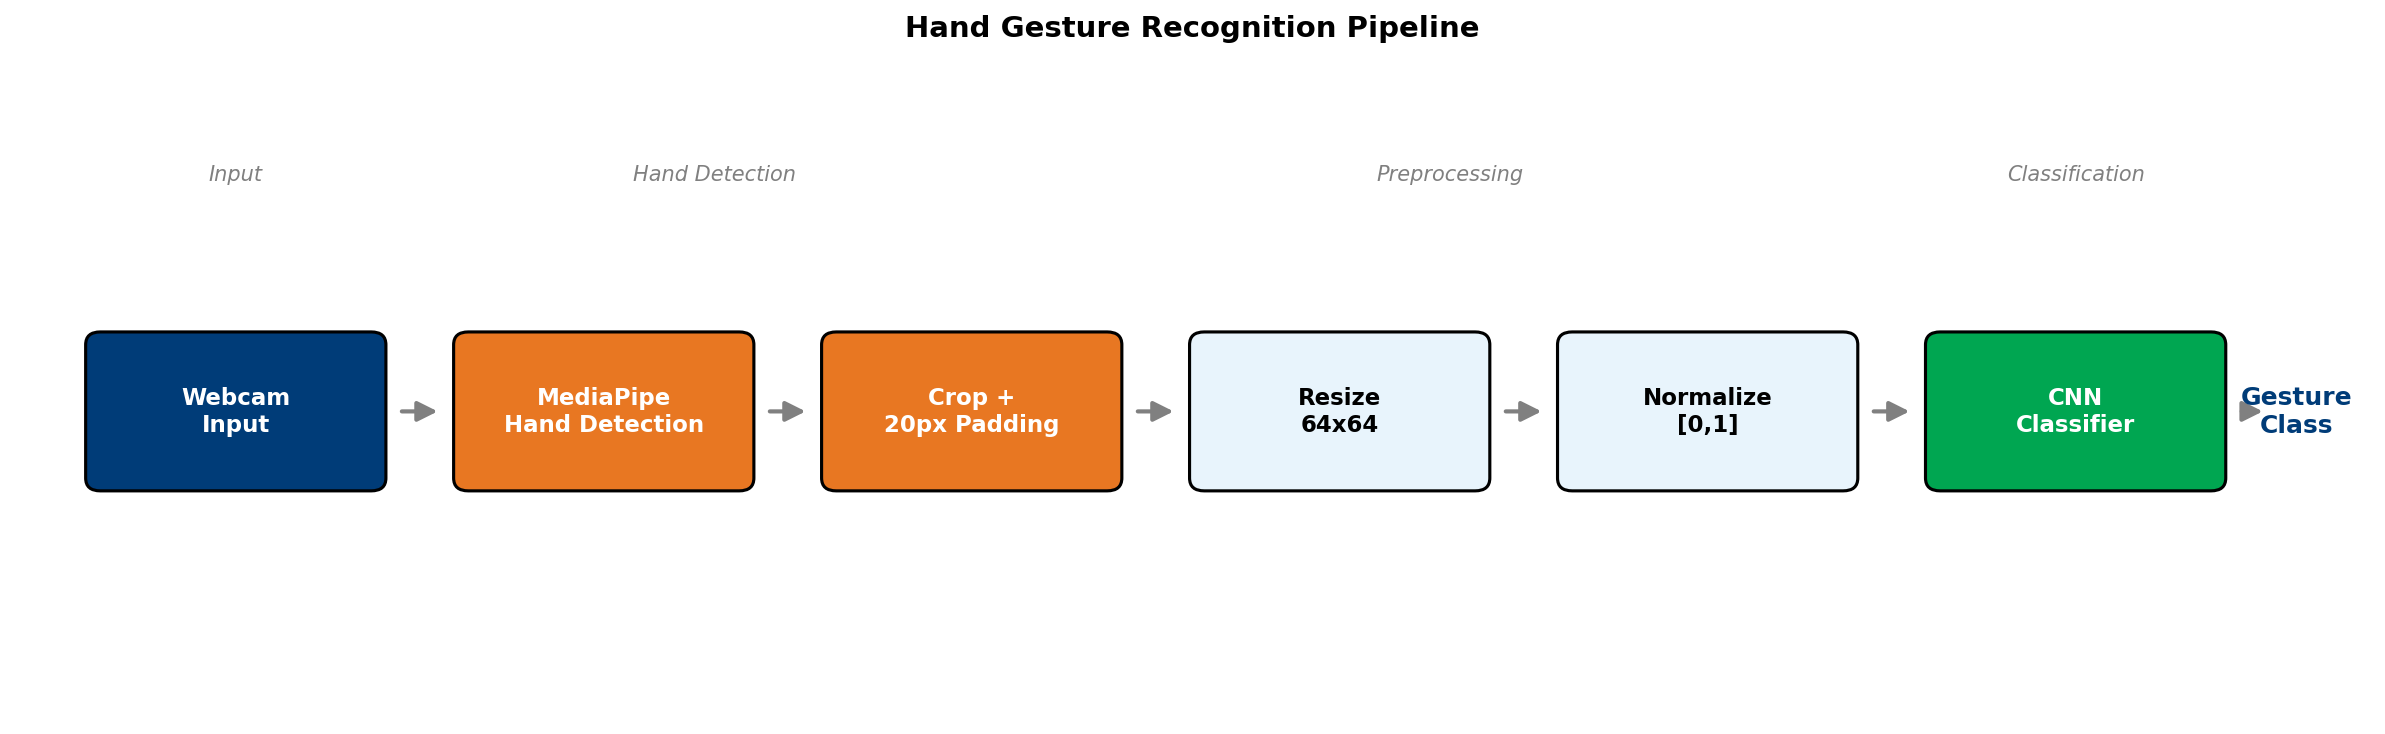
\includegraphics[width=\textwidth]{images/pipeline.png}
    \vspace{0.5cm}

    % Three columns for the details below
    \begin{columns}[T, onlytextwidth]
        \column{0.31\textwidth}
            \textbf{MediaPipe Hands}
            \footnotesize
            \begin{itemize}
                 \item Detects 21 hand landmarks (fingertips, knuckles, palm).
            \end{itemize}

        \column{0.31\textwidth}
            \textbf{Bounding Box}
            \footnotesize
            \begin{itemize}
                \item Extract hand region with 20px padding.
            \end{itemize}

        \column{0.31\textwidth}
            \textbf{Result}
            \footnotesize
            \begin{itemize}
                \item CNN only sees the hand, not the background.
            \end{itemize}
    \end{columns}
\end{frame}

% --- Slide 5: CNN Architecture ---
\begin{frame}{CNN Architecture: SimpleCNN}
    \centering
    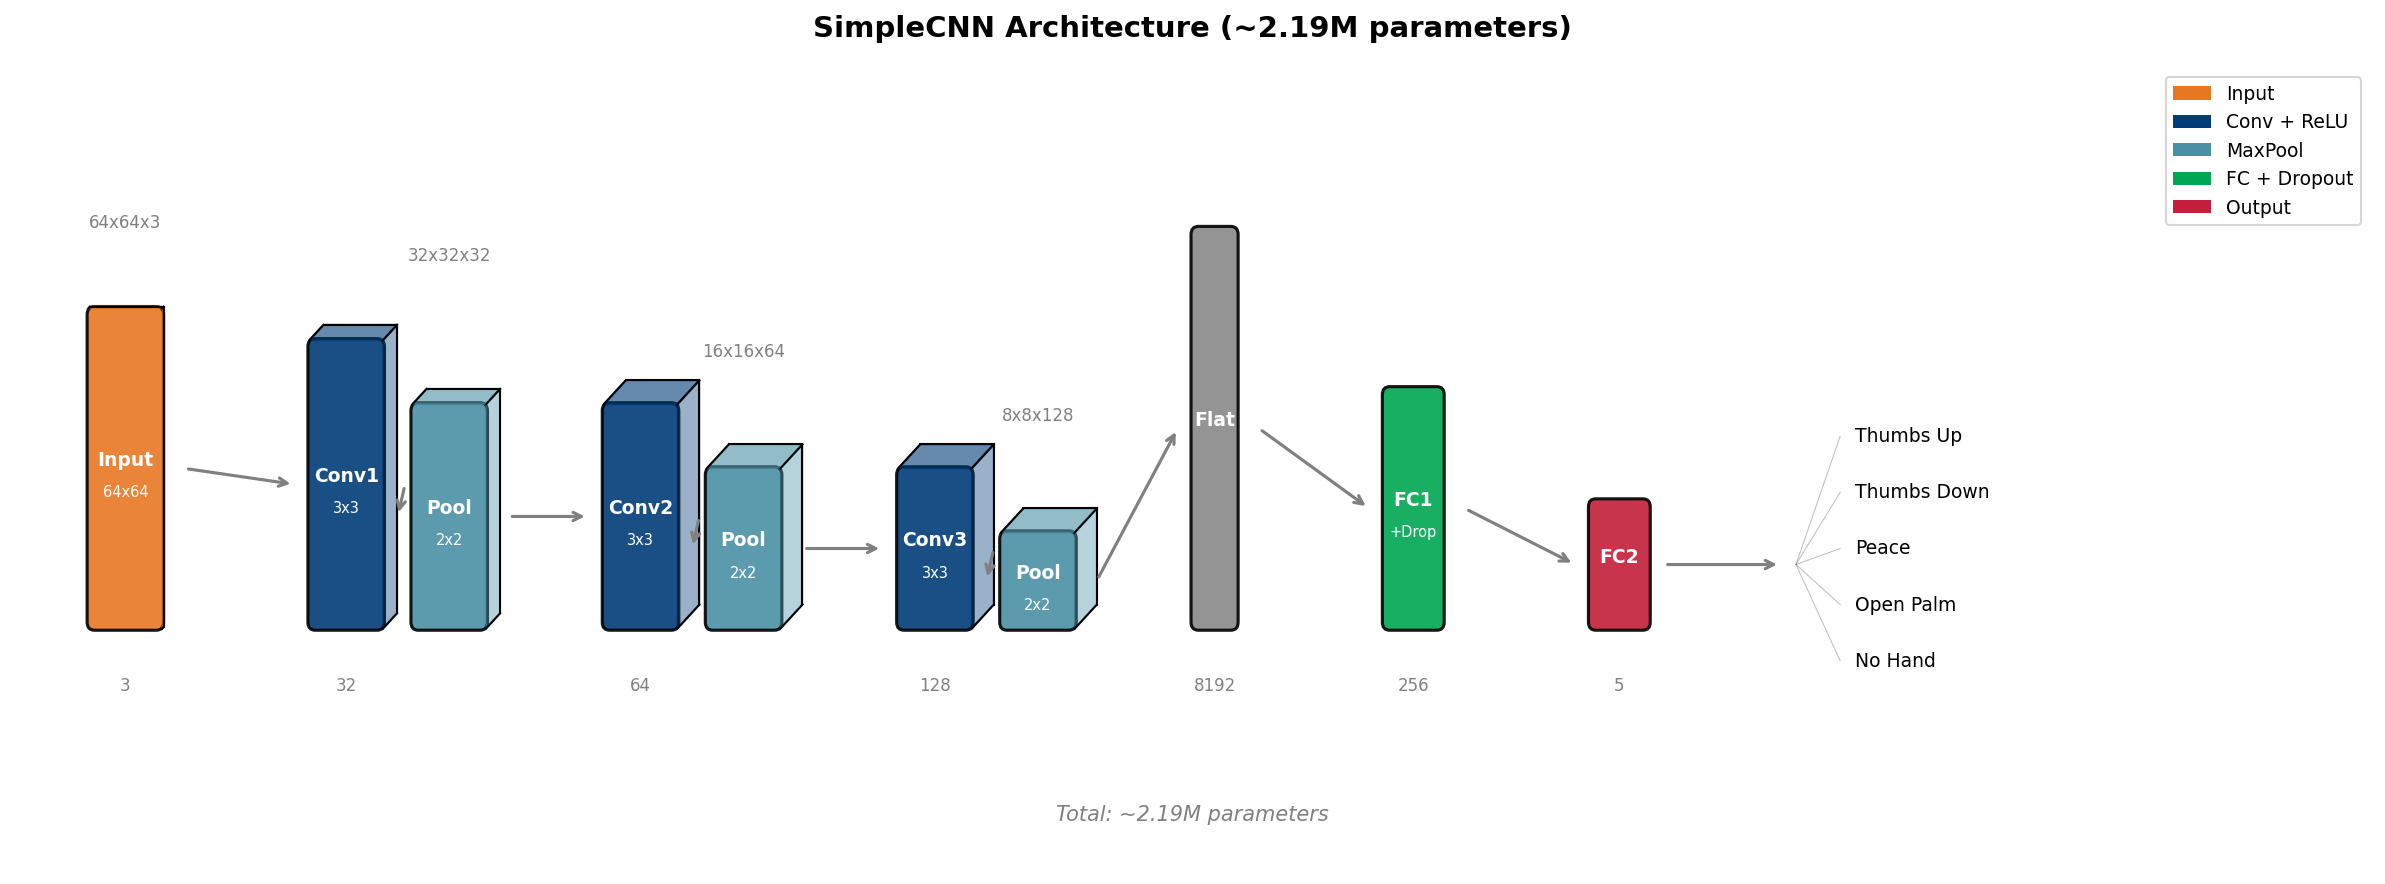
\includegraphics[width=\textwidth, height=0.45\textheight, keepaspectratio]{images/architecture.png}
    \vspace{0.2cm}

    \begin{columns}[T, onlytextwidth]
        \column{0.48\textwidth}
            \textbf{Structure:}
            \begin{itemize}
                \item 3 Conv blocks ($3 \to 32 \to 64 \to 128$)
                \item 2 FC layers ($8192 \to 256 \to 5$)
                \item Dropout (50\%) for regularization
            \end{itemize}

        \column{0.48\textwidth}
            \textbf{Details:}
            \begin{itemize}
                \item Input: $64 \times 64$ RGB
                \item Total: $\sim 2.19$M parameters
                \item ReLU activations
            \end{itemize}
    \end{columns}
\end{frame}

% --- Slide 6: Data Augmentation ---
\begin{frame}{Data Augmentation Strategy}
    \centering
    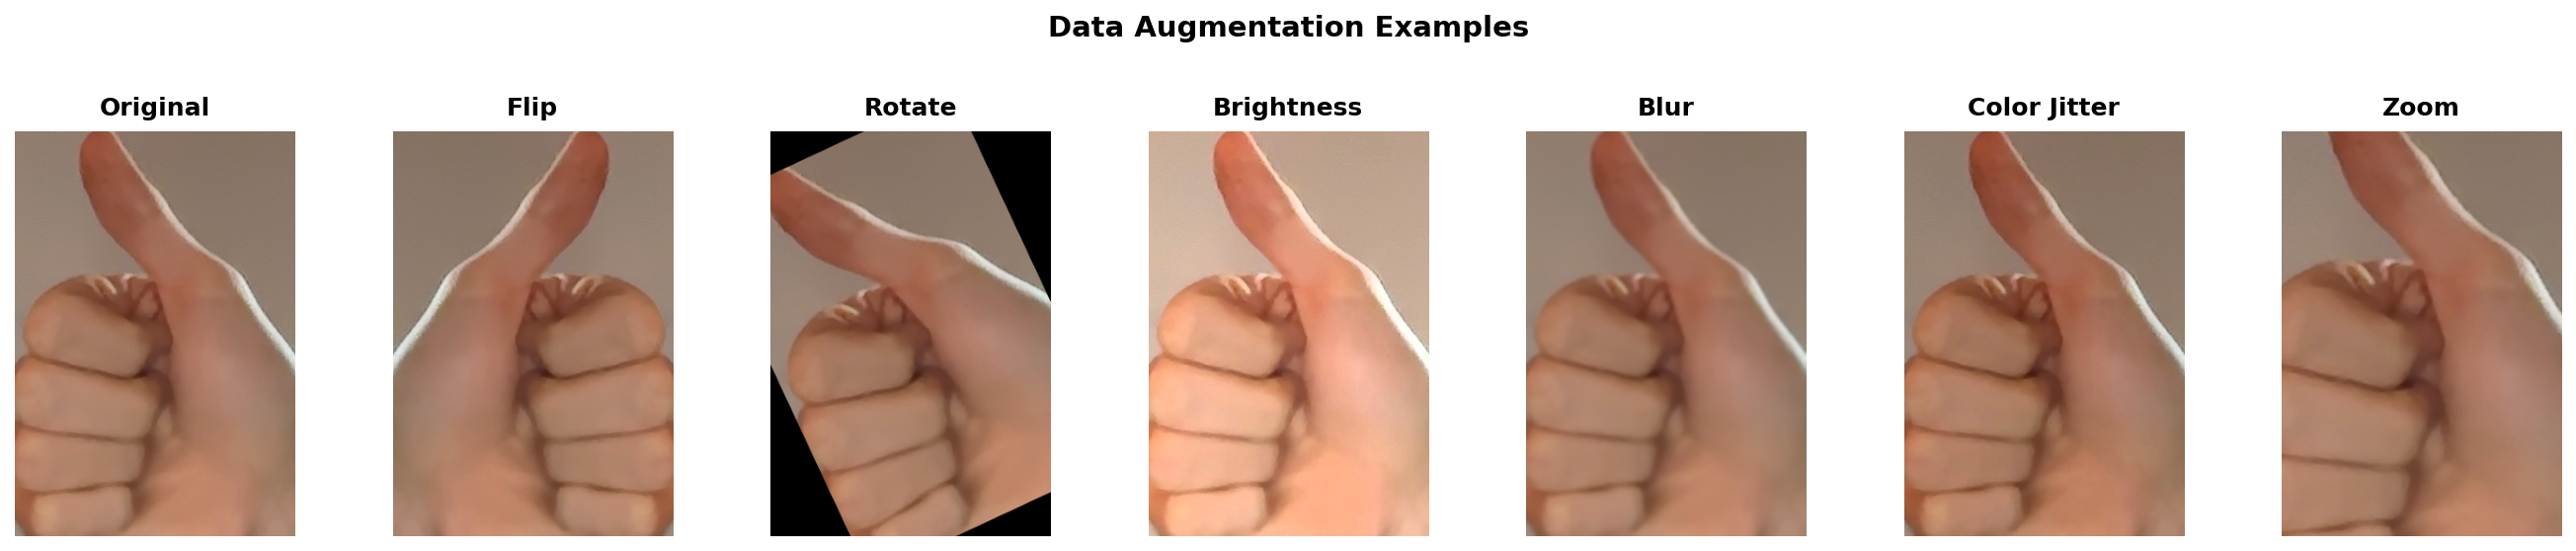
\includegraphics[width=0.95\textwidth, height=3cm, keepaspectratio]{images/augmentation_examples.png}
    \vspace{0.3cm}

    \begin{columns}[T, onlytextwidth]
        \column{0.48\textwidth}
            \textbf{6 Custom OpenCV Augmentations:}
            \begin{itemize}
                \item Horizontal flip
                \item Rotation ($\pm 30^{\circ}$)
                \item Brightness ($0.5\times$--$1.5\times$)
                \item Gaussian blur ($k=3,5,7$)
                \item Color jitter (HSV)
                \item Zoom ($1.0\times$--$1.3\times$)
            \end{itemize}

        \column{0.48\textwidth}
            \textbf{Application:}
            \begin{itemize}
                \item 50\% probability per sample
                \item Training only (not test)
                \item No \texttt{torchvision} -- all hand-rolled
            \end{itemize}
    \end{columns}
\end{frame}

% --- Slide 7: Experimental Setup ---
\begin{frame}{Experimental Setup}
    \begin{columns}[T, onlytextwidth]
        \column{0.5\textwidth}
            \textbf{Two Experiment Sets:}
            \begin{enumerate}
                \item \textbf{Augmentation Comparison:}
                \begin{itemize}
                    \item No augmentation (baseline)
                    \item Single augmentations
                    \item Flip + Rotate combined
                    \item All augmentations
                \end{itemize}
                \vspace{0.2cm}
                \item \textbf{Dataset Size Impact:}
                \begin{itemize}
                    \item 50 / 100 / 200 / Full samples per class
                    \item With and without augmentation
                \end{itemize}
            \end{enumerate}

        \column{0.45\textwidth}
            \textbf{Training Configuration:}
            \begin{table}
                \centering
                \begin{tabular}{ll}
                    \toprule
                    Parameter & Value \\
                    \midrule
                    Optimizer & Adam \\
                    Learning rate & 0.001 \\
                    Epochs & 20 \\
                    Batch size & 32 \\
                    Split & 80/20 \\
                    Seed & 42 \\
                    \bottomrule
                \end{tabular}
            \end{table}
            \small
            $\sim$300 images per class\\ (collected via webcam)
    \end{columns}
\end{frame}

% --- Slide 8: Results (Augmentation) ---
\begin{frame}{Results: Augmentation Comparison}
    \begin{columns}[c, onlytextwidth]
        \column{0.6\textwidth}
            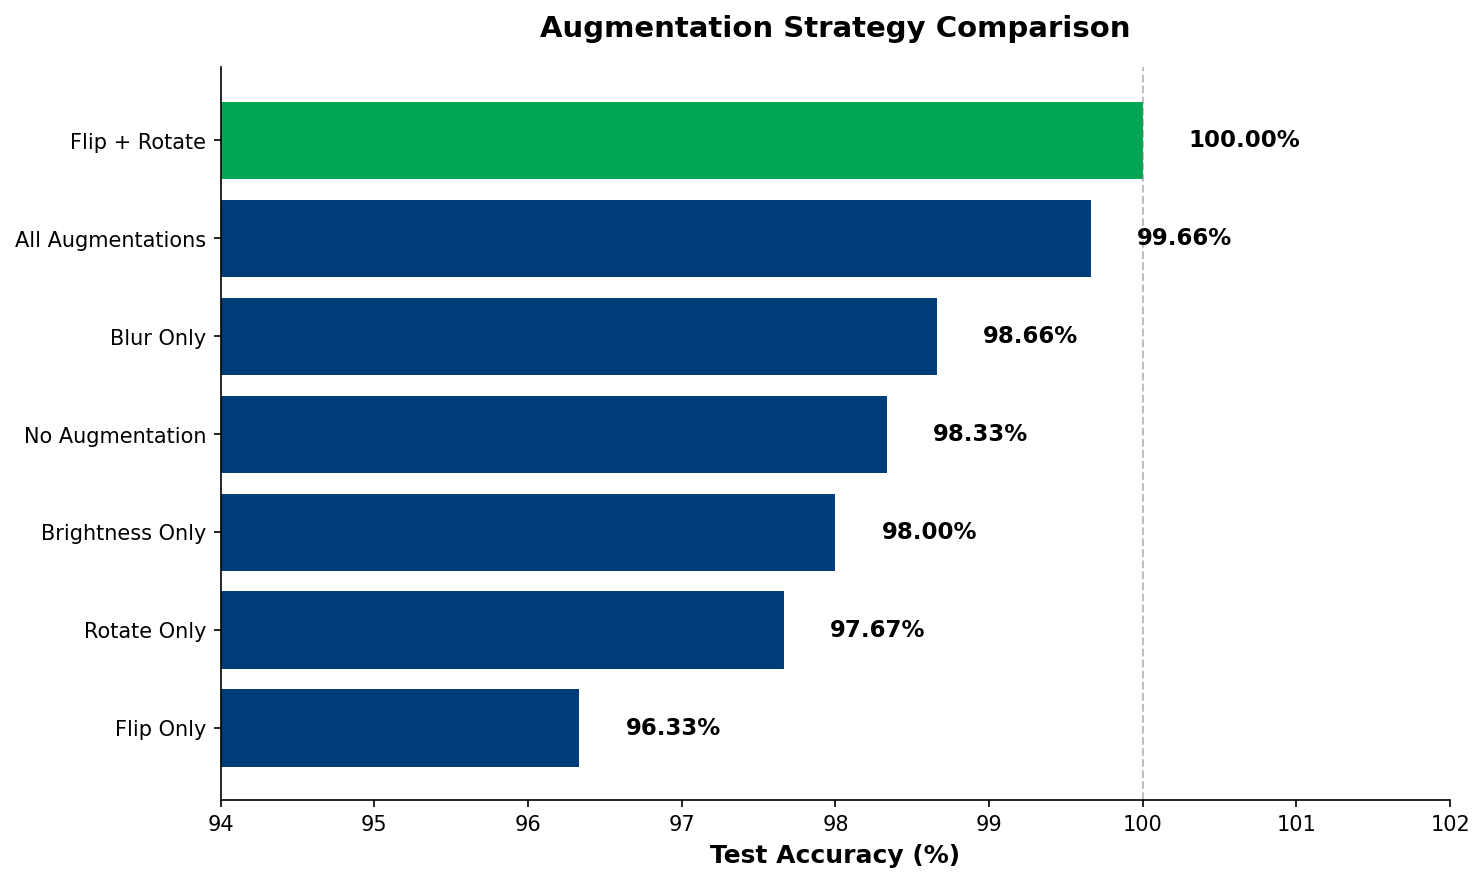
\includegraphics[width=\textwidth]{images/augmentation_comparison.png}

        \column{0.35\textwidth}
            \textbf{Key Finding:}
            \begin{alertblock}{Flip + Rotate = 100\%}
            \end{alertblock}
            Surprisingly, \textit{all augmentations} (99.67\%) performed \textbf{worse} than flip+rotate alone.
            \vspace{0.4cm}
            \textbf{Why?}
            \begin{itemize}
                \item Geometric transforms match real gesture variation.
                \item Too many augmentations add noise.
                \item \textit{``More is not always better.''}
            \end{itemize}
    \end{columns}
\end{frame}

% --- Slide 9: Results (Dataset Size) ---
\begin{frame}{Results: Dataset Size Impact}
    \begin{columns}[c, onlytextwidth]
        \column{0.6\textwidth}
            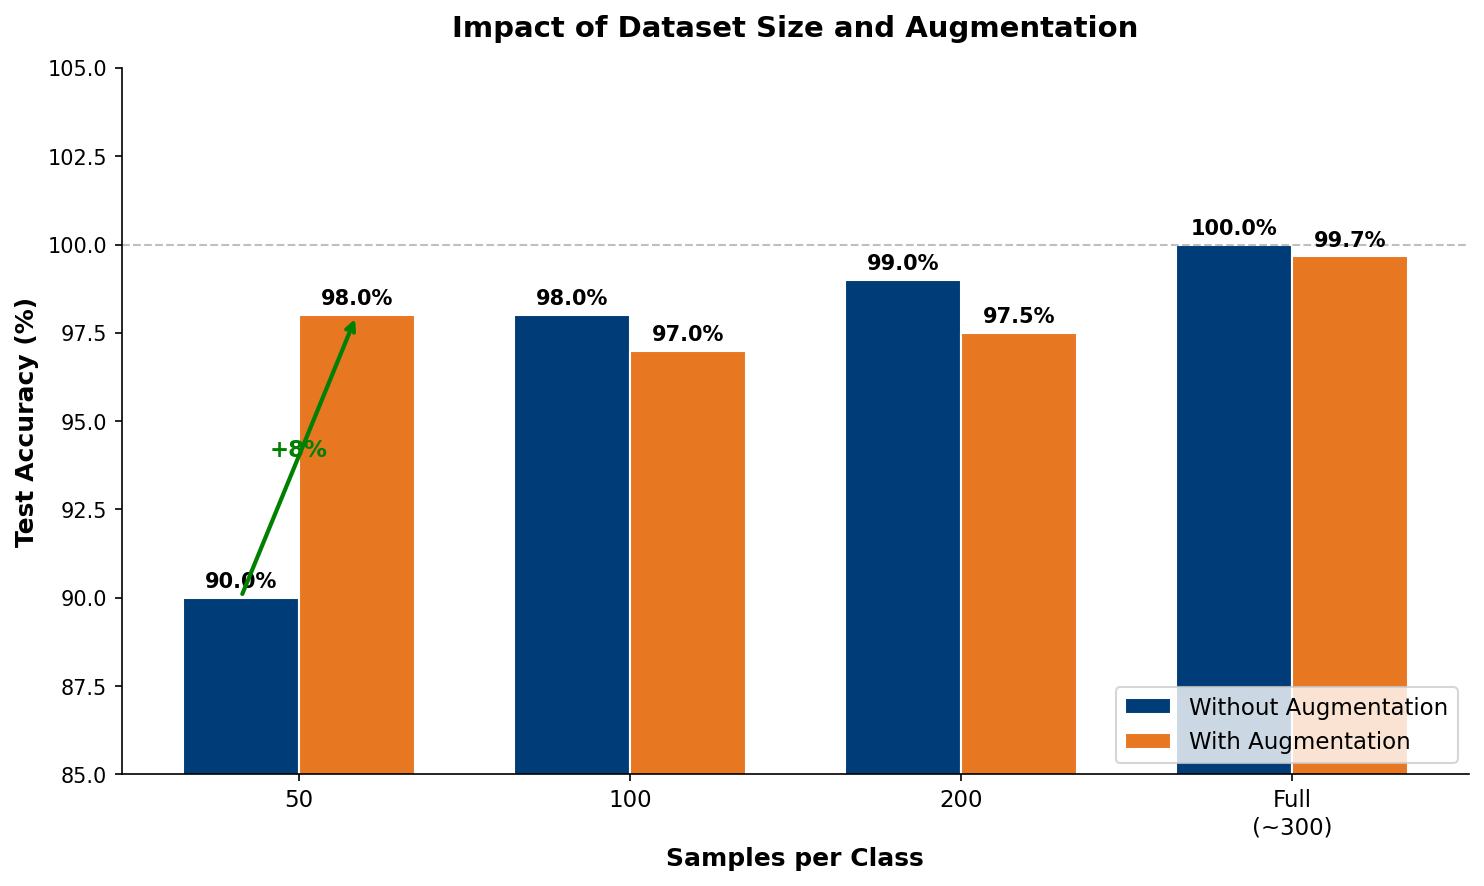
\includegraphics[width=\textwidth]{images/dataset_size_effect.png}

        \column{0.35\textwidth}
            \textbf{Key Finding:}
            Augmentation helps most with \alert{small data}.

            \vspace{0.3cm}
            \begin{itemize}
                \item \textbf{50 samples:} $90\% \to 98\%$ \\ \alert{(+8\% improvement)}
                \item \textbf{Full data:} Augmentation matters less.
                \item 100\% possible without augmentation (if data is sufficient).
            \end{itemize}

            \vspace{0.3cm}
            \textbf{Practical Insight:}
            Augmentation is crucial when data is limited.
    \end{columns}
\end{frame}

% --- Slide 10: Training Dynamics ---
\begin{frame}{Training Dynamics}
    \centering
    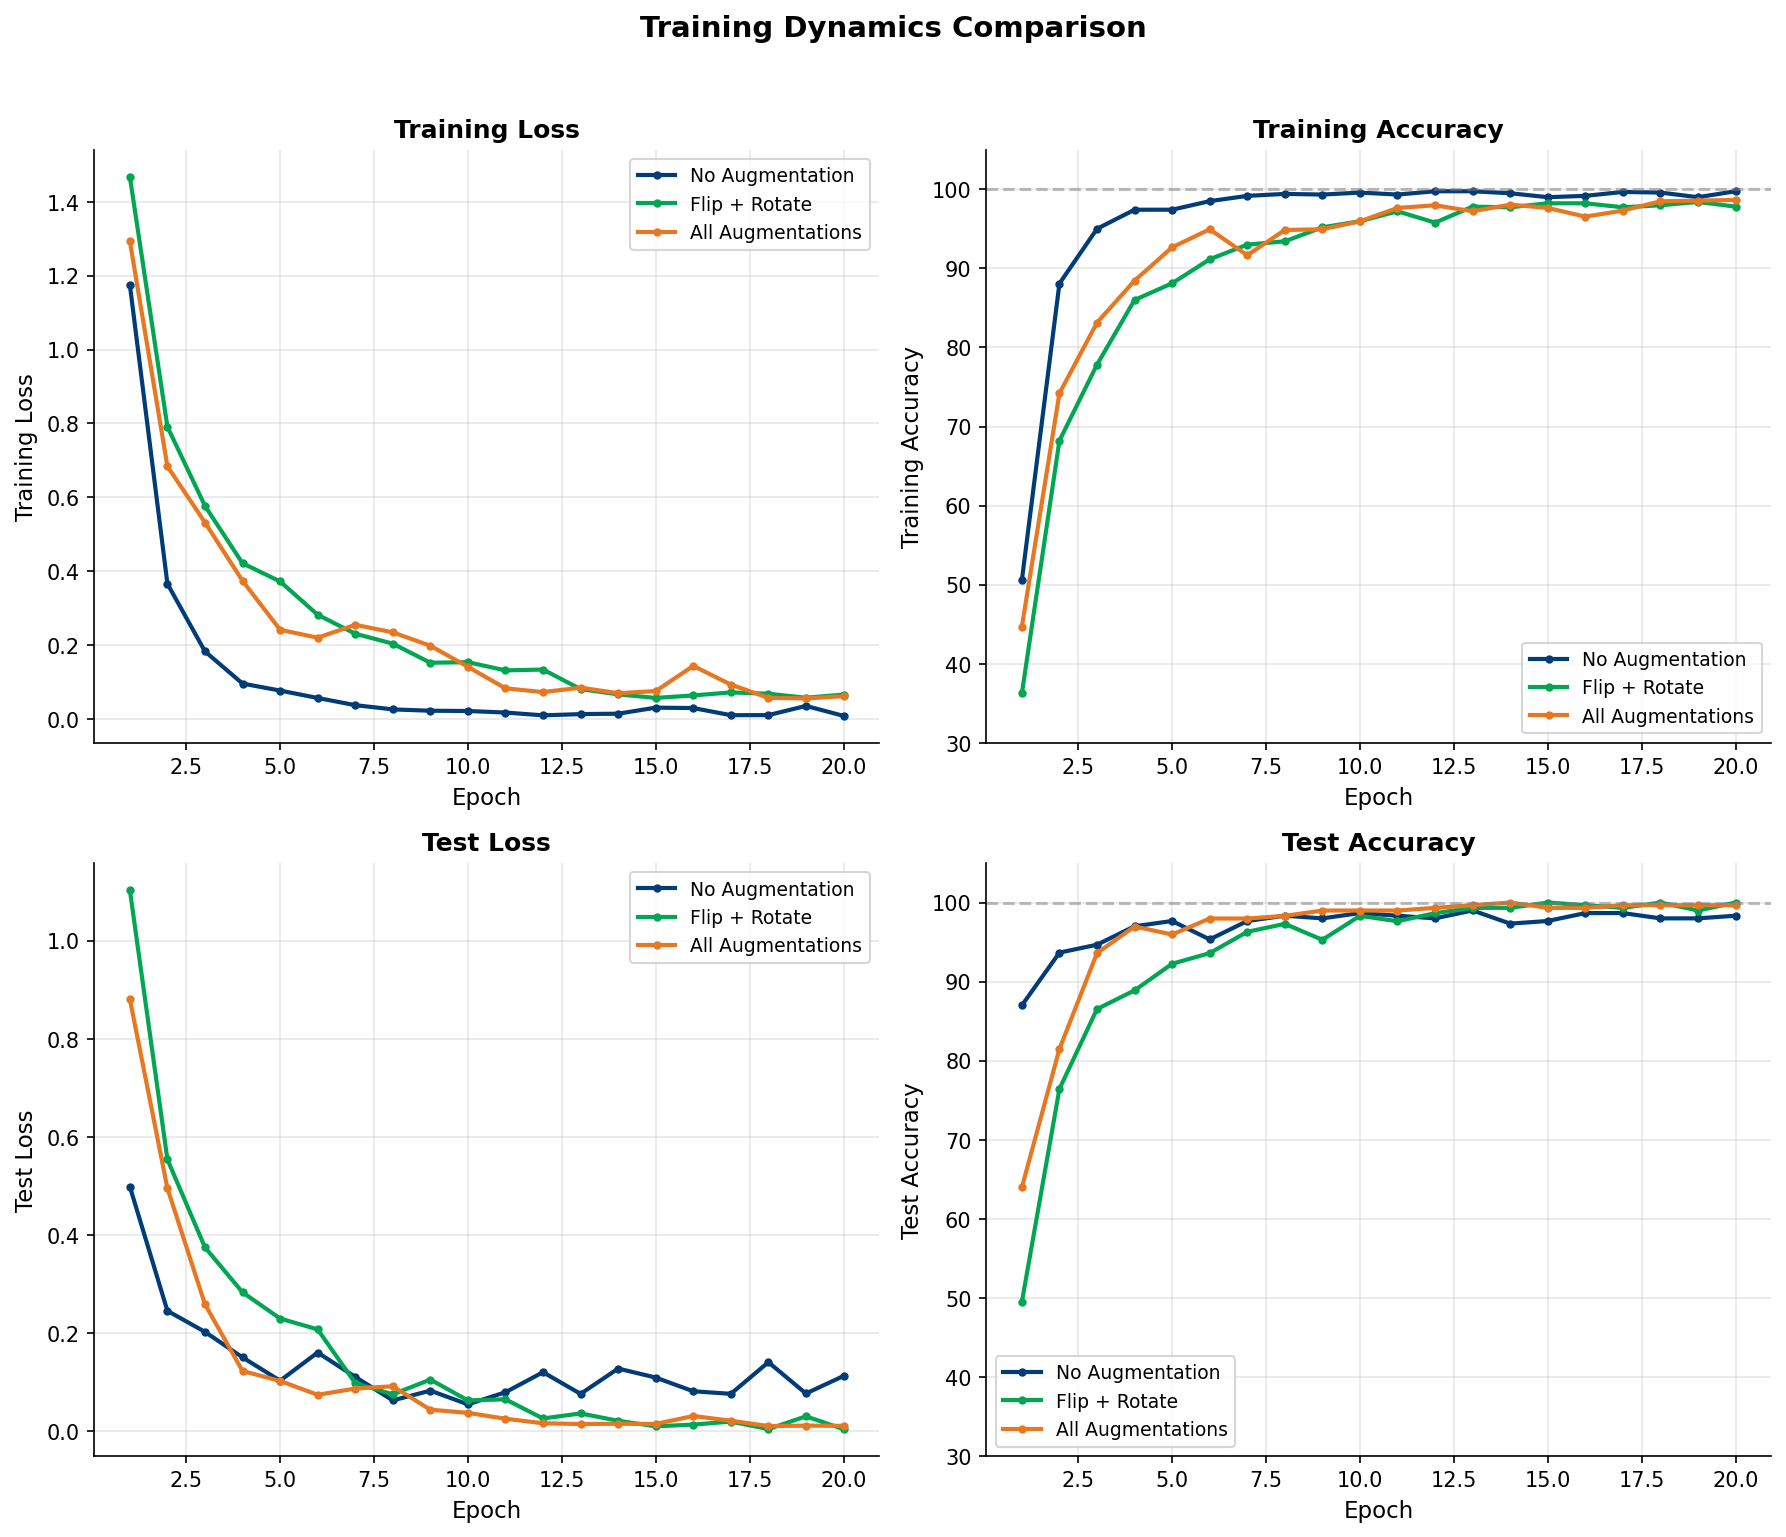
\includegraphics[width=0.95\textwidth, height=0.8\textheight, keepaspectratio]{images/training_curves.png}
\end{frame}

% --- Slide 11: Final Performance ---
\begin{frame}{Final Model Performance}
    \begin{columns}[c, onlytextwidth]
        \column{0.5\textwidth}
            \centering
            
\includegraphics[width=0.9\textwidth]{images/confusion_matrix.png}
            \captionof*{figure}{\footnotesize Confusion Matrix: Perfect Classification}

        \column{0.45\textwidth}
            \textbf{Best Model: Flip + Rotate}
            \begin{itemize}
                \item \alert{100\% test accuracy}
                \item No misclassifications
                \item Real-time inference on webcam
                \item Robust across lighting conditions
            \end{itemize}

            \vspace{1cm}
            \textbf{Model saved as:}
            \texttt{\small models/model\_flip\_rotate.pth}
    \end{columns}
\end{frame}

% --- Slide 12: Takeaways ---
\begin{frame}{Key Takeaways \& Limitations}
    \begin{columns}[T, onlytextwidth]
        \column{0.48\textwidth}
            \textbf{What Worked:}
            \begin{enumerate}
                \item \textbf{Hand cropping was crucial} \\ \footnotesize Isolate the signal from noise.
                \item \textbf{Domain-relevant augmentation} \\ \footnotesize Flip + rotate match real variation.
                \item \textbf{Simple architecture} \\ \footnotesize 3 conv layers sufficient for 5 classes.
            \end{enumerate}

            \vspace{0.3cm}
            \textbf{Counterintuitive:}
            More augmentation $\neq$ better results.
        \column{0.48\textwidth}
            \textbf{Limitations:}
            \begin{itemize}
                \item Only 5 gesture classes.
                \item Single hand detection.
                \item Trained on limited subjects (may not generalize to all hands).
                \item Requires good lighting for MediaPipe.
            \end{itemize}

            \vspace{0.3cm}
            \textbf{Future Work:}
            \begin{itemize}
                \item More gesture classes.
                \item Multi-hand support.
                \item Diverse training data.
            \end{itemize}
    \end{columns}
\end{frame}

% --- Slide 13: Live Demo ---
{
\setbeamercolor{background canvas}{bg=uibkblue}
\setbeamercolor{normal text}{fg=white}
\begin{frame}
    % We enforce white color explicitly here to be safe against theme overrides
    \color{white}
    \centering

    \vspace{2.5cm}
    {\Huge \textbf{Live Demo}}

    \vspace{2.5cm}
    \textbf{Tim Dedie \& Nick Somitsch} \\
    University of Innsbruck
\end{frame}
}

\end{document}